% Report, Assignment 2b: multimodal emotion recognition on TESS
% Build (from this folder): xelatex report.tex  (run twice)
\documentclass[11pt,a4paper]{article}
\usepackage{fontspec}
\usepackage[margin=2.0cm]{geometry}
\usepackage{graphicx,booktabs,caption,enumitem,float,tabularx,array,amsmath}
\usepackage[hidelinks]{hyperref}
\setmainfont{Cambria}
\setmonofont{Consolas}[Scale=0.86]
\newcommand{\code}[1]{\texttt{#1}}
\graphicspath{{../Results/plots/}}
\setlist{itemsep=1pt,topsep=3pt}
\captionsetup{font=small,labelfont=bf}
\setlength{\parskip}{3pt}
\emergencystretch=2em

\title{Multimodal emotion recognition on TESS:\\ speech, text and fusion\\[3pt]\large Assignment 2b report}
\author{Simhaa T.\,T.}
\date{November 2026}

\begin{document}
\maketitle

\section{Summary}
I built three emotion classifiers for the Toronto emotional speech set (TESS): one that hears the speech, one that
reads the transcript, and one that fuses both. Each follows the assignment's blocks: preprocessing, feature
extraction, temporal or contextual modelling, fusion and a classifier. Frozen pretrained encoders (WavLM Base+ for
speech, BERT for text) extract the features, and small trained heads do the rest.

The dataset decides most of the story. Every TESS clip says ``Say the word \emph{X}'', and each sentence occurs
once in every emotion, so \textbf{the text carries no information about the emotion}. I proved this three ways: no
text-only classifier can beat 1/7 (14.3\%) on TESS, a pretrained text-emotion model scores exactly that, and our
text model does too. The fusion models therefore lean entirely on speech: replacing their speech with another
clip's drops them to chance, while replacing their text changes nothing.

On sentences never seen in training, speech alone recognises 99.8\% of clips. On an unseen \emph{speaker}, accuracy
falls to 60--65\%. The learned representations still separate the new speaker's emotions into clean clusters
(96\% cluster purity for YAF), but the classifier names some clusters wrongly; a single labelled clip per emotion
from the new speaker lifts accuracy from 65\% to 92\%. Speaker augmentation (pitch and speed changes of the training
voice) adds 20 points to log-mel features but little to WavLM, which already generalises across voices; there it
mainly makes training stable. Two of my additions did not work as intended and I report them as found: per-speaker feature normalisation lowered cross-speaker accuracy, and cross-modal attention learned
a sharp pooling over time rather than a word-to-audio alignment, although that made it the most noise-robust model.

\section{Data, and why the text cannot help}
TESS holds recordings of two actresses, OAF (aged 64) and YAF (aged 26), each saying ``Say the word \emph{X}'' for
200 target words in seven emotions: angry, disgust, fear, happy, neutral, pleasant surprise (``ps'') and sad. That
gives 2,800 clips. The Kaggle copy stores the dataset twice in nested folders, so the loader removes duplicates by
file name; one file is misnamed (\code{OA\_bite\_neutral.wav}) and was skipped, leaving 2,799 clips. The labels come
from the file names, and the transcript is the carrier sentence with the target word.

\paragraph{An upper bound for every text model.} A text classifier sees only the sentence, so it must give every
clip of the same sentence the same answer. Each sentence occurs once per emotion and speaker, so whatever it
answers is right for at most one clip in seven. The best possible text-only accuracy on TESS is therefore
$\sum_{\text{sentences}} \max_{\text{emotion}} n / N = 14.3\%$ (computed from the data:
\code{Results/text\_zero\_shot.json}). A model that beats this is reading something other than the text, such as a
leak through the file order or the split.

\paragraph{Splits.} The splits are built so that results cannot come from memorising sentences or voices.
\begin{table}[H]\centering\small
\caption{Data splits. All seven emotions stay balanced in every part.}
\label{tab:splits}
\begin{tabularx}{\linewidth}{@{}l>{\raggedright\arraybackslash}Xrrr@{}}
\toprule
Split & Rule & Train & Val. & Test \\
\midrule
Unseen words & the 200 words split 140 / 30 / 30, both speakers in every part; test sentences never occur in
training & 1,959 & 420 & 420 \\
OAF $\to$ YAF & train and validate on OAF (validation on 30 held-out words), test on all of YAF & 1,189 & 210 &
1,400 \\
YAF $\to$ OAF & the reverse & 1,190 & 210 & 1,399 \\
\bottomrule
\end{tabularx}
\end{table}

\section{Architecture decisions}
\begin{table}[H]\centering\small
\caption{The blocks of each pipeline. Encoders in the feature-extraction row stay frozen; everything below them
trains (0.8--2.1\,M parameters).}
\label{tab:arch}
\begin{tabularx}{\linewidth}{@{}l>{\raggedright\arraybackslash}X>{\raggedright\arraybackslash}X@{}}
\toprule
Block & Speech & Text \\
\midrule
Preprocessing & mono 16\,kHz; leading and trailing silence trimmed (30\,dB below the peak); peak-normalised; at
most 4\,s (TESS clips: 1.1--3.0\,s after trimming, mean 2.0\,s) & lower case, punctuation removed, WordPiece
tokens of BERT (\code{[CLS] say the word X [SEP]}) \\
Feature extraction & WavLM Base+ hidden states of all 13 layers, 50 frames/s, 768-d; log-mel (64 bands) as an
ablation & BERT base hidden states of all 13 layers, 768-d per token \\
Temporal / contextual modelling & learned softmax weights over the 13 layers; linear projection to 256; 2-layer
BiLSTM (128 per direction); attention pooling & learned layer weights; projection to 256; one Transformer encoder
layer (4 heads); attention pooling \\
Fusion & \multicolumn{2}{>{\raggedright\arraybackslash}p{0.665\linewidth}}{gated multimodal unit (GMU) on the two
256-d vectors; ablations: concatenation, and cross-modal attention in which every text token attends over the
speech frames} \\
Classifier & \multicolumn{2}{l}{256 $\to$ 128 $\to$ 7, ReLU, dropout 0.3, softmax} \\
\bottomrule
\end{tabularx}
\end{table}

\paragraph{Preprocessing.} WavLM was trained on 16\,kHz audio, so I resample to 16\,kHz (TESS is 24.4\,kHz) rather
than feed it a rate it never saw. Silence at the ends carries no emotion and only adds frames to pad, so I trim it.
Peak normalisation removes recording-level differences while keeping loudness \emph{changes} inside a clip, which
do carry emotion. For text, BERT's own tokeniser is the right preprocessing because the frozen encoder expects it.

\paragraph{Speech features: WavLM Base+.} Emotion lives in how something is said: pitch, energy, tempo, voice
quality. Self-supervised speech models learn these cues without labels, and WavLM Base+ leads the emotion task
of the SUPERB benchmark among base-size models. Its layers hold different information (acoustic near the bottom,
phonetic higher up), so rather than pick one, the model learns a weighted sum of all 13. The learned weights stay
close to uniform with a slight lean to the lower layers (0.083 for layer 0 down to 0.071 for layer 10), which fits
emotion being an acoustic rather than a phonetic property. A 64-band log-mel spectrogram, the classic hand-made
feature, serves as the ablation.

\paragraph{Temporal modelling: BiLSTM with attention pooling.} Emotion unfolds over the clip, for example a rising
pitch in surprise or a falling, slow ending in sadness. A bidirectional LSTM reads the frame sequence in both
directions, and attention pooling lets the model weight the frames that matter (the stressed target word, say)
instead of averaging everything. TESS has only about 2,000 training clips, so a small recurrent model fits better
than a deep Transformer.

\paragraph{Text features and contextual modelling: BERT + one Transformer layer.} BERT gives contextual word
vectors and a learned layer mix lets the model choose among its layers. One trainable self-attention layer adapts
them to the task and attention pooling summarises the sentence. On a dataset whose text carries emotion this is a
reasonable design; on TESS it has nothing to learn, which is the point of Section~\ref{sec:fusion}.

\paragraph{Fusion: gated multimodal unit.} The GMU (Arevalo et al., 2017) learns, for each clip and each dimension,
how much of the fused vector to take from each modality: $z = \sigma(W[s;t])$,
$h = z \odot \tanh(W_s s) + (1-z) \odot \tanh(W_t t)$. It can ignore a useless modality, and its gate $z$ shows how
much it relies on speech. Two ablations test the choice: plain concatenation, and cross-modal attention, my
addition, in which every text token queries the speech frames. The idea was that the text cannot tell the
emotion but can tell the model where in the audio to listen.

\paragraph{Training.} AdamW (learning rate $10^{-3}$, weight decay $10^{-2}$), batch 32, cross-entropy with label
smoothing 0.05, at most 40 epochs, keeping the epoch with the best validation macro-F1 (patience 8; runs stopped
after 9--19 epochs). Every variant runs with seeds 0, 1 and 2, on a Kaggle T4 GPU; the whole experiment, including
feature extraction, took 70 minutes.

\section{Experiments: speech-only, text-only, multimodal}
\begin{table}[H]\centering\small
\caption{Test accuracy and macro-F1 (\%), mean $\pm$ standard deviation over 3 seeds. Chance is 14.3\%.}
\label{tab:main}
\setlength{\tabcolsep}{4.5pt}
\begin{tabular}{@{}lrrrrrr@{}}
\toprule
 & \multicolumn{2}{c}{Unseen words} & \multicolumn{2}{c}{OAF $\to$ YAF} & \multicolumn{2}{c}{YAF $\to$ OAF} \\
Model & Acc. & F1 & Acc. & F1 & Acc. & F1 \\
\midrule
\textbf{Speech} (WavLM) & \textbf{99.8} $\pm$ 0.2 & 99.8 & \textbf{65.4} $\pm$ 7.3 & 62.3 & \textbf{60.2} $\pm$ 1.9 & 52.4 \\
Speech, log-mel & 99.4 $\pm$ 0.3 & 99.4 & 32.2 $\pm$ 4.3 & 28.0 & 35.9 $\pm$ 1.4 & 26.3 \\
Speech, speaker-normalised & 99.9 $\pm$ 0.1 & 99.9 & 56.4 $\pm$ 4.2 & 53.7 & 51.3 $\pm$ 1.5 & 45.6 \\
\textbf{Text} (BERT) & 14.3 $\pm$ 0.0 & 3.6 & 14.3 $\pm$ 0.0 & 3.6 & 14.3 $\pm$ 0.0 & 3.6 \\
\textbf{Fusion} (GMU) & 99.1 $\pm$ 0.1 & 99.1 & 59.5 $\pm$ 11.2 & 56.7 & 57.0 $\pm$ 2.7 & 50.8 \\
Fusion, concat & 99.8 $\pm$ 0.1 & 99.8 & 57.6 $\pm$ 11.1 & 54.1 & 45.9 $\pm$ 8.1 & 37.4 \\
Fusion, cross-attention & 99.5 $\pm$ 0.2 & 99.5 & 52.1 $\pm$ 12.4 & 50.0 & 52.1 $\pm$ 1.7 & 44.7 \\
\bottomrule
\end{tabular}
\end{table}

\begin{itemize}
\item \textbf{Speech is almost perfect when the voice is known.} On unseen words the WavLM model makes 2 errors in
1,260 test predictions (3 seeds $\times$ 420). The task becomes hard only for a new voice: 65\% and 60\%.
\item \textbf{Text sits exactly at the bound.} 14.3\% in every split, and macro-F1 3.6\% because each seed's model
settles on one constant answer. A pretrained text-emotion classifier
(\code{j-hartmann/}\allowbreak\code{emotion-english-distilroberta-base}) also scores exactly 14.3\%: it calls 87.5\% of the sentences
neutral and the rest mostly disgust or anger (``Say the word \emph{nag}'' 0.96 disgust), judging the target word's
meaning, which has nothing to do with how the actress spoke it.
\item \textbf{Fusion never beats speech.} On unseen words all fusion models stay within a point of speech; across
speakers they lose 3--14 points. The text branch adds parameters and noise but no information.
\item \textbf{The pretrained features matter most for new voices.} Log-mel features reach 99.4\% on known voices
but only 32--36\% across speakers, half the WavLM result: self-supervised pretraining on thousands of speakers is
what lets the model generalise to a voice it never heard.
\end{itemize}

\section{Analysis}
\subsection{Which emotions are easiest and hardest?}
With a known voice every emotion is easy (recall $\geq$ 99.4\%). Across speakers the differences are large:
\begin{table}[H]\centering\small
\caption{Recall per emotion of the speech model (\%, mean over 3 seeds).}
\label{tab:recall}
\begin{tabular}{@{}lrrrrrrr@{}}
\toprule
Split & angry & disgust & fear & happy & neutral & ps & sad \\
\midrule
Unseen words & 100.0 & 100.0 & 100.0 & 100.0 & 99.4 & 99.4 & 100.0 \\
OAF $\to$ YAF & 17.2 & 73.3 & 97.8 & 16.3 & 99.3 & 56.7 & 97.2 \\
YAF $\to$ OAF & 13.3 & 95.2 & 99.7 & 12.5 & 97.0 & 7.7 & 96.5 \\
\bottomrule
\end{tabular}
\end{table}

\begin{figure}[H]\centering
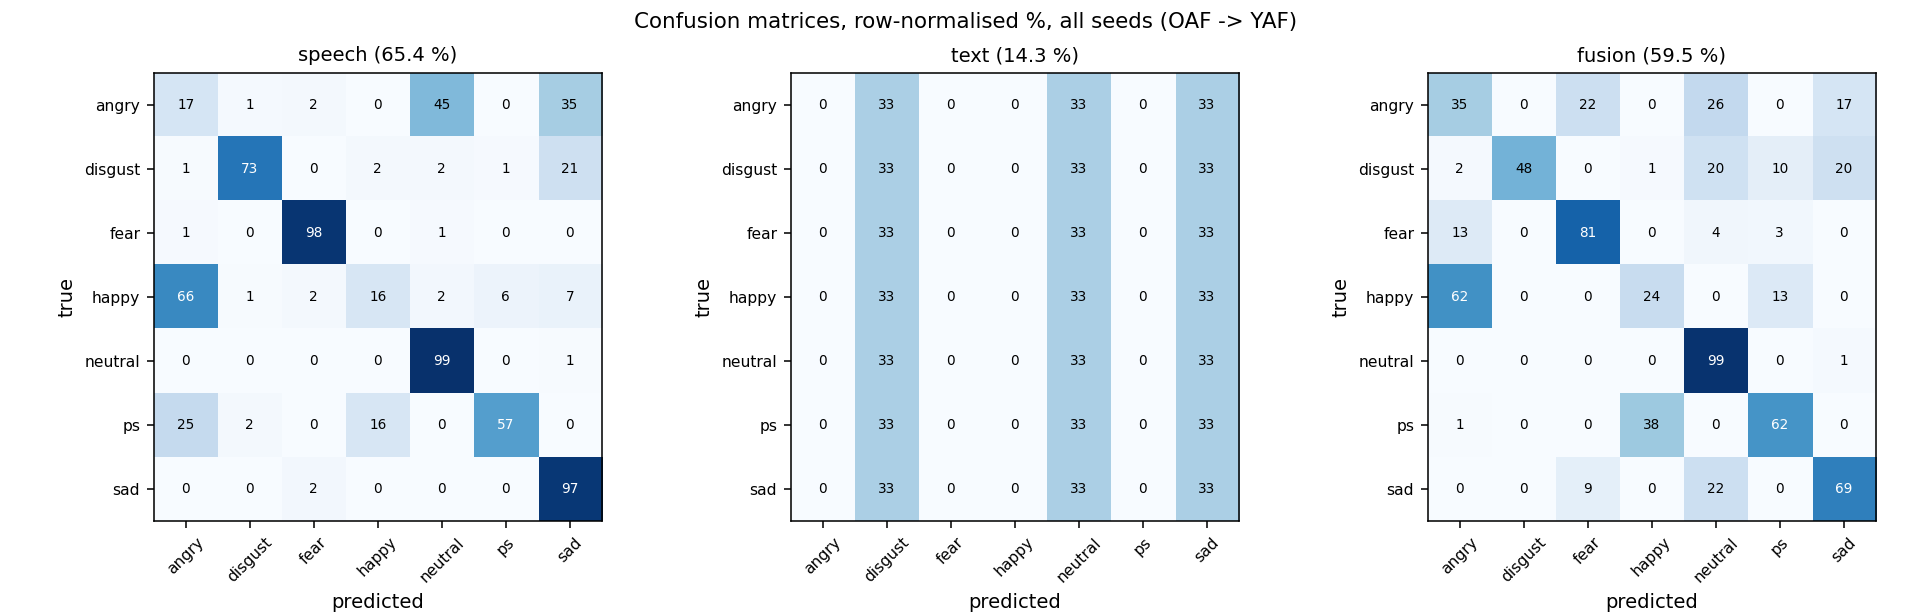
\includegraphics[width=\linewidth]{confusion_oaf2yaf.png}\\[2pt]
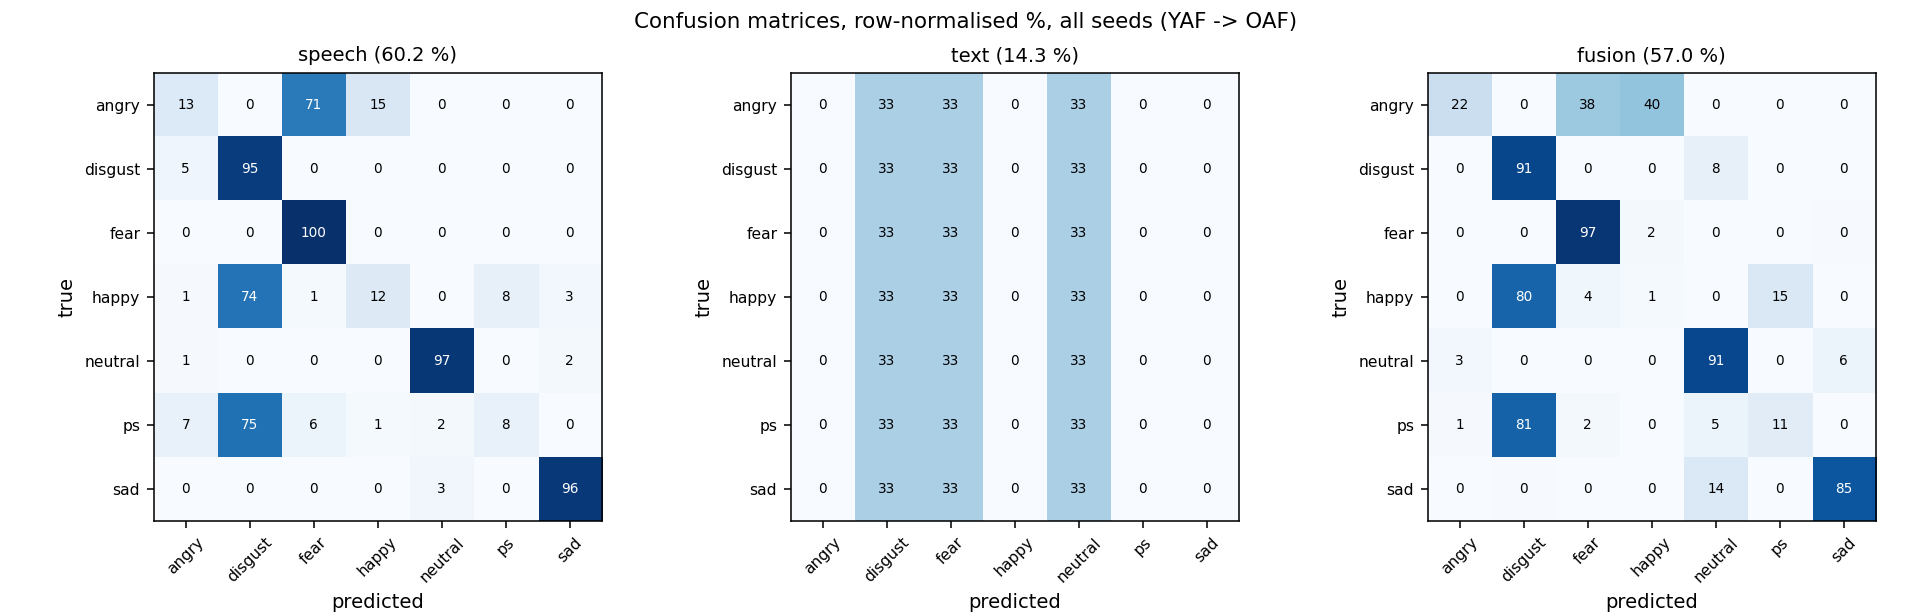
\includegraphics[width=\linewidth]{confusion_yaf2oaf.png}
\caption{Confusion matrices of the cross-speaker tests, summed over seeds and row-normalised.}
\label{fig:conf}
\end{figure}

\textbf{Easiest: fear, neutral and sad} transfer to the other speaker almost perfectly (96--100\%). These are
likely the emotions whose delivery both actresses share most: in the usual description of emotional speech,
neutral is flat, sad slow, low and quiet, and fear high and tense. \textbf{Hardest: angry, happy and pleasant
surprise}, at 8--57\%. All three are high-arousal emotions, typically loud, fast and high-pitched, so they differ
mainly in voice quality and the shape of the pitch contour, which individual speakers realise differently. The errors are
systematic rather than random (Figure~\ref{fig:conf}). Trained on OAF, the model hears 66\% of YAF's happy clips as
angry; trained on YAF, it hears 71\% of OAF's angry clips as fear and three quarters of OAF's happy and surprised
clips as disgust. A whole emotion of the new speaker lands on one wrong category, usually with high confidence
(median 0.85 for YAF happy $\to$ angry). Section~\ref{sec:fewshot} shows what this means.

\subsection{When does fusion help most?}
\label{sec:fusion}
\begin{table}[H]\centering\small
\caption{Fusion models with one modality replaced by that of a random other test clip (accuracy, \%).}
\label{tab:shuffle}
\begin{tabular}{@{}llrrr@{}}
\toprule
Fusion & Split & Both intact & Speech shuffled & Text shuffled \\
\midrule
GMU & unseen words & 99.1 & 12.5 & 99.1 \\
GMU & OAF $\to$ YAF & 59.5 & 13.0 & 59.5 \\
GMU & YAF $\to$ OAF & 57.0 & 14.4 & 57.0 \\
Concatenation & unseen words & 99.8 & 12.7 & 99.8 \\
Cross-modal attention & unseen words & 99.5 & 12.7 & 99.5 \\
\bottomrule
\end{tabular}
\end{table}

\paragraph{On TESS, never, and the models know it.} Shuffling the text leaves every fusion model's accuracy
unchanged (within 0.1 point, in every split and seed); shuffling the speech drops it to chance
(Table~\ref{tab:shuffle}). The GMU gate takes 83--85\% of the fused vector from speech, with little difference
between emotions (0.81--0.86). The fusion models
learnt on their own to ignore the text, which is the correct response to Section 2's bound.

\paragraph{When fusion would help.} Fusion helps when the two modalities carry \emph{complementary} information:
when the words themselves express emotion (``I'm furious'', ``what a lovely day''), when the voice is ambiguous,
or when one channel is degraded and the other is not. Datasets of natural conversation such as IEMOCAP or MELD have
this property and fusion gains there are well documented. TESS controls the text on purpose to isolate the voice,
so it is the one setting where a text branch must contribute nothing.

\paragraph{Noise: a gain that is not fusion.} I added white noise to the test speech at 20, 10 and 0\,dB SNR
(unseen words). Speech alone falls to 50.3\% at 0\,dB, the GMU to 44.9\%, but the cross-modal attention model keeps
70.6\% ($\pm$ 11.9). Its text is shuffle-proof, so the gain cannot come from the words: the attention layer acts
as a second, sharper pooling over the speech frames (Section~\ref{sec:neg}), which copes better with noise.

\begin{figure}[H]\centering
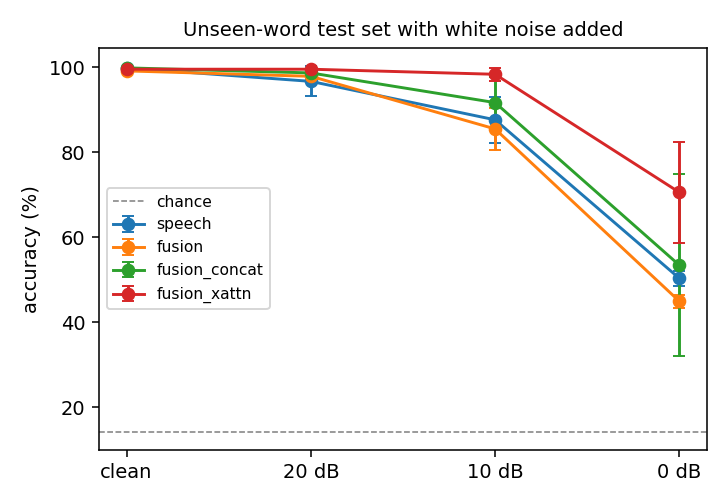
\includegraphics[width=0.62\linewidth]{noise_robustness.png}
\caption{Accuracy on the unseen-word test set with white noise added to the speech (mean and SD over seeds).}
\label{fig:noise}
\end{figure}

\subsection{Error analysis: five failure cases}
\begin{table}[H]\centering\small
\caption{Five failure cases. Confidence is the predicted class's softmax probability; ``words'' is the unseen-word
split, O$\to$Y and Y$\to$O the cross-speaker splits.}
\label{tab:fail}
\begin{tabularx}{\linewidth}{@{}lllll>{\raggedright\arraybackslash}X@{}}
\toprule
Clip & Model & Split & True & Predicted & What it shows \\
\midrule
\code{OAF\_hall\_ps} & speech & words & surprise & disgust (0.81) & one of only two speech errors in 1,260 unseen-word
predictions, and fairly confident; I found no pattern behind it \\
\code{OAF\_mode\_neutral} & speech, GMU & words & neutral & sad (0.61, 0.52) & the only clip both models get wrong,
with low confidence: it sits between the two low-arousal emotions \\
\code{YAF\_knock\_neutral} & GMU & words & neutral & sad (0.98) & the speech model gets it right; the fusion model,
with its idle text branch, is confidently wrong: the cost of a modality without information \\
\code{YAF\_puff\_happy} & speech & O$\to$Y & happy & angry (0.98) & one of 394 such errors: YAF's happy clips land
where OAF's angry clips were in training \\
\code{OAF\_soup\_angry} & speech & Y$\to$O & angry & fear (0.96) & one of 428 such errors: OAF's angry clips land
where YAF's fearful clips were \\
\bottomrule
\end{tabularx}
\end{table}

The first three are isolated: borderline clips between neighbouring emotions, and one error that the fusion model
adds. The last two are not mistakes about single clips but about a whole emotion of a new speaker, made with
high confidence, which a confidence threshold could not catch.

\subsection{Separability of the learned representations}
\begin{figure}[H]\centering
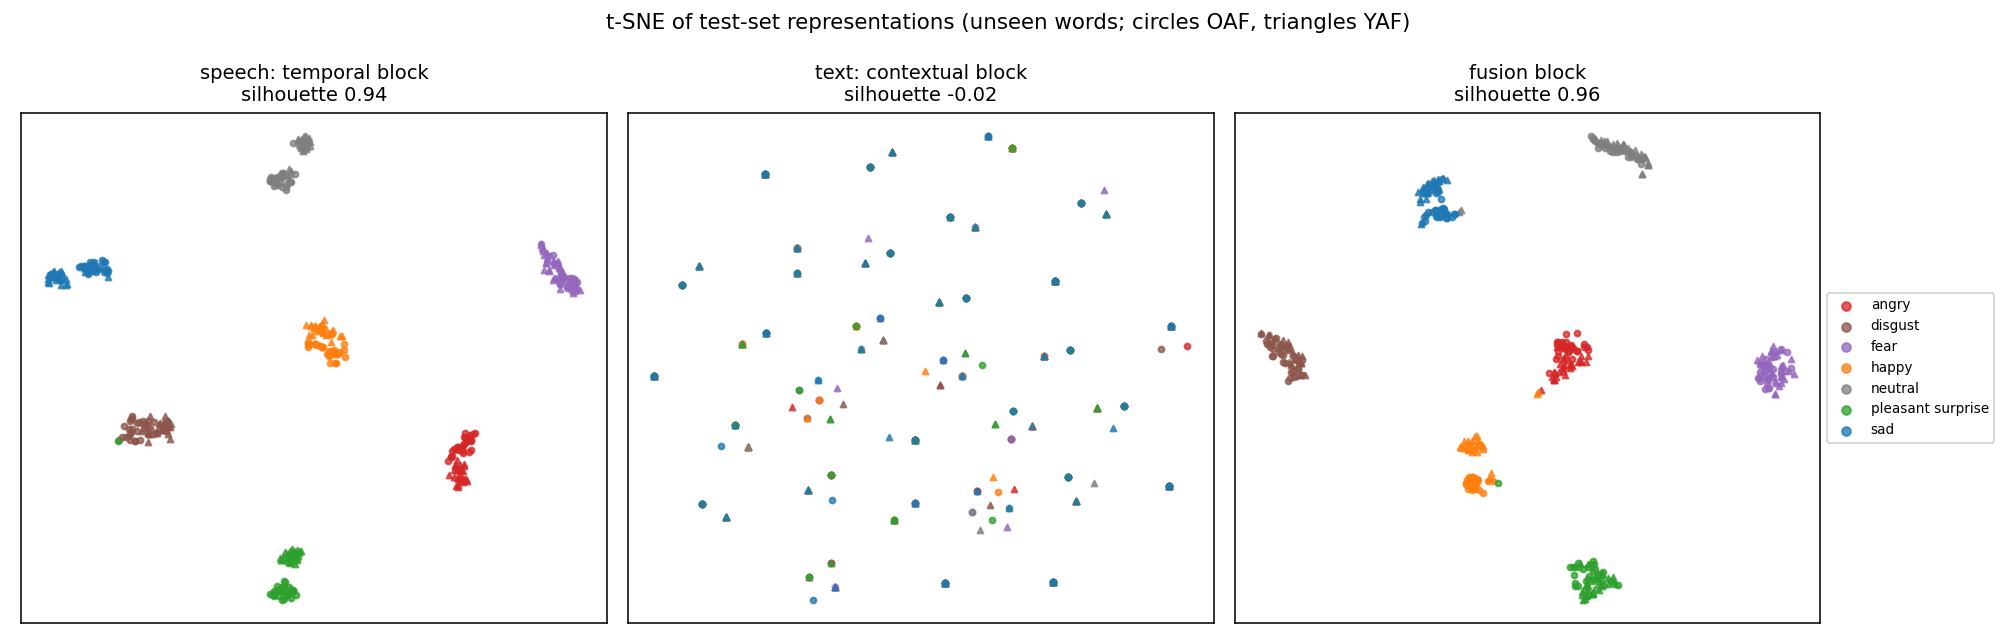
\includegraphics[width=\linewidth]{tsne_word.png}\\[2pt]
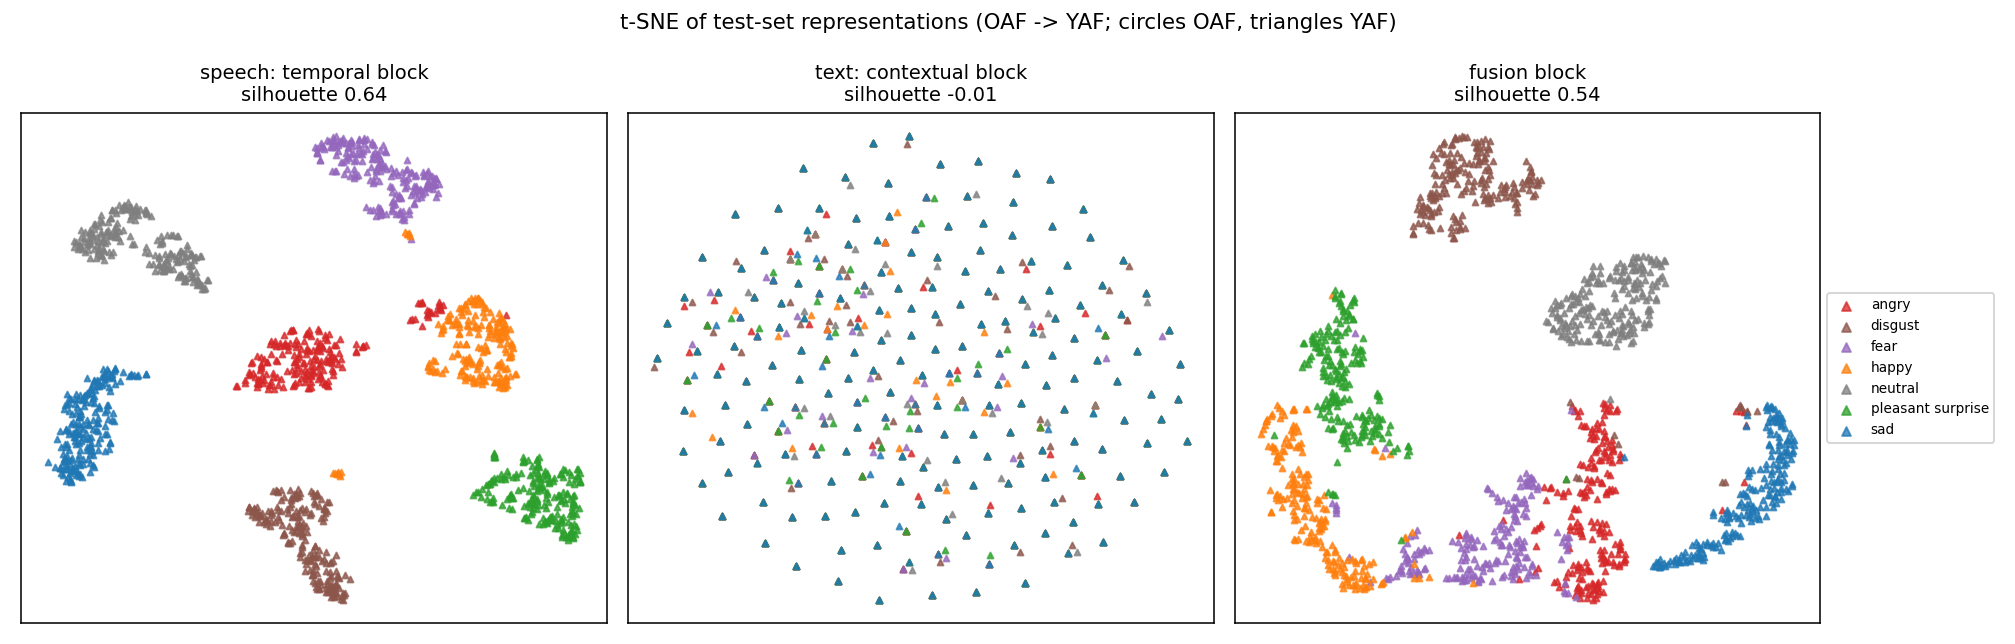
\includegraphics[width=\linewidth]{tsne_oaf2yaf.png}
\caption{t-SNE of the test-set outputs of the temporal block (speech model), the contextual block (text model)
and the fusion block (GMU), seed 0. Top: unseen words; bottom: OAF $\to$ YAF, where all test clips are YAF's.}
\label{fig:tsne}
\end{figure}

\begin{table}[H]\centering\small
\caption{Silhouette score of each block's output (cosine, by emotion; 1 = perfectly separated, 0 = no structure),
mean of 3 seeds.}
\label{tab:sil}
\begin{tabular}{@{}lrrr@{}}
\toprule
Block & Unseen words & OAF $\to$ YAF & YAF $\to$ OAF \\
\midrule
Temporal (speech model) & 0.94 & 0.64 & 0.48 \\
Contextual (text model) & $-$0.02 & $-$0.01 & $-$0.01 \\
Fusion (GMU) & 0.96 & 0.54 & 0.44 \\
\bottomrule
\end{tabular}
\end{table}

With known voices, the temporal and fusion blocks form seven tight, separate clusters, each mixing both speakers.
The contextual block shows no emotion structure at all: points with the same target word coincide whatever the
emotion. On the unseen speaker the temporal block still forms seven compact clusters (silhouette 0.64), even though
the classifier labels a third of them wrongly. The fusion block separates them less well (0.54): the idle text
branch blurs them.

\subsection{Adapting to a new speaker with a handful of labels}
\label{sec:fewshot}
The clusters of Figure~\ref{fig:tsne} suggest the cross-speaker errors come from naming, not from the
representation. I tested this on the saved test representations (\code{scripts/few\_shot\_adaptation.py}).
\emph{Cluster purity} groups the new speaker's clips into 7 clusters with k-means, using no labels, and counts how
many land in a cluster that a one-to-one match assigns to their emotion. \emph{Few-shot} trains a logistic
regression on $k$ labelled clips per emotion of the new speaker and tests on the rest (20 random draws per $k$ and
seed).

\begin{table}[H]\centering\small
\caption{Accuracy on the unseen speaker (\%, speech model, mean $\pm$ SD over seeds).}
\label{tab:fewshot}
\begin{tabular}{@{}lrrrrr@{}}
\toprule
 & Model as trained & Cluster purity (no labels) & $k = 1$ & $k = 2$ & $k = 5$ \\
\midrule
OAF $\to$ YAF & 65.4 $\pm$ 7.3 & 96.2 $\pm$ 0.9 & 92.3 $\pm$ 1.6 & 95.4 $\pm$ 2.2 & 97.9 $\pm$ 0.8 \\
YAF $\to$ OAF & 60.2 $\pm$ 1.9 & 87.4 $\pm$ 1.5 & 78.9 $\pm$ 2.3 & 86.5 $\pm$ 1.5 & 91.5 $\pm$ 1.7 \\
\bottomrule
\end{tabular}
\end{table}

\begin{figure}[H]\centering
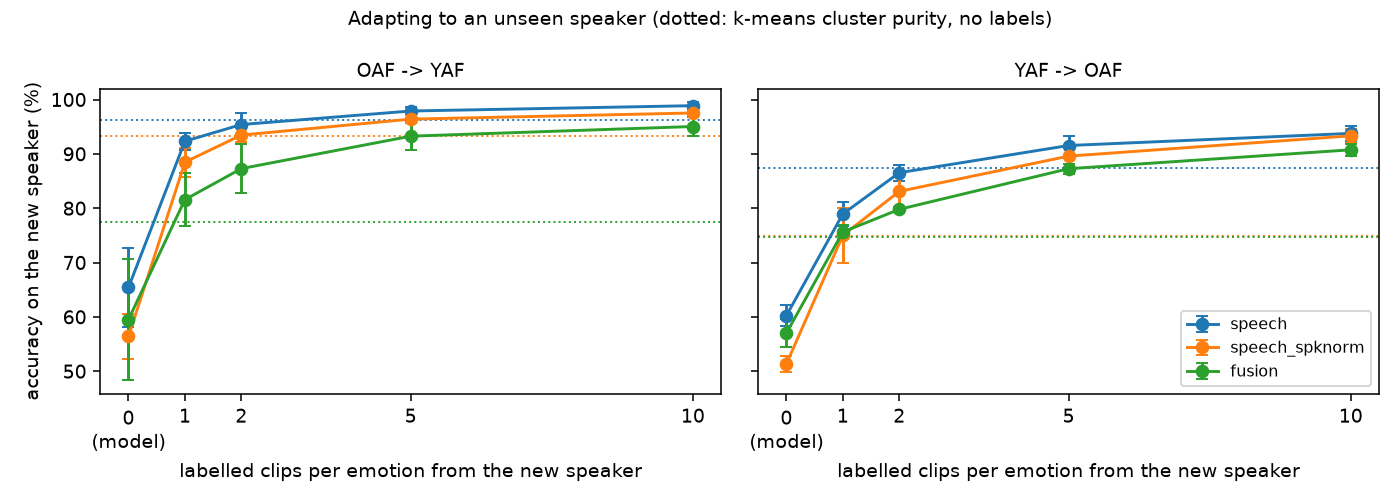
\includegraphics[width=0.9\linewidth]{few_shot_adaptation.png}
\caption{Accuracy on the unseen speaker against the number of labelled clips per emotion; dotted lines show the
cluster purity reached without labels.}
\label{fig:fewshot}
\end{figure}

The representation already separates the new speaker's emotions: 96\% of YAF's clips fall into the right cluster
without a single label. \textbf{Seven labelled clips, one per emotion, raise accuracy from 65\% to 92\%} for YAF and
from 60\% to 79\% for OAF; five per emotion reach 98\% and 92\%. A deployed system would therefore not need to
retrain on a new voice, only to recalibrate its last layer with a few examples.

\paragraph{Zero labels are not enough.} I also tried naming the new speaker's clusters without any labels: k-means
clusters, each given the emotion with the highest mean log-probability under the model, one emotion per cluster
(TESS is balanced). It did not help reliably: 64.6\% ($\pm$ 9.2) for YAF and 68.8\% ($\pm$ 16.2) for OAF, with
single seeds ranging from 48\% to 88\%. The model is confidently wrong about whole clusters, so its own
probabilities cannot name them; a handful of true labels can. Averaging the three seeds' predictions (an ensemble)
reaches 100\% on unseen words but changes little across speakers (68.0\% and 59.5\%;
\code{Results/seed\_ensemble.csv}). YAF $\to$ OAF stays harder in every
column: OAF's angry, happy and surprised clips overlap more in the representation, and her clusters are less
pure (87\%).

\subsection{Speaker augmentation}
\label{sec:aug}
The model fails on a new voice because it heard only one during training. Speaker augmentation gives it more:
every training clip of the training speaker also enters training in four altered versions, pitch-shifted by
$\pm$3 semitones and played 0.9 and 1.1 times as fast (resampling, which scales pitch, formants and tempo together,
roughly like a different vocal tract). Validation and test clips stay unaltered. To fit five versions of every clip
in memory, these runs use the mean of WavLM's 13 layers instead of the learned mix (justified by the near-uniform
layer weights), and the same run trains the unaugmented controls on identical features
(\code{kaggle/TESS\_augmentation.ipynb}, \code{Results\_aug/}). The log-mel control reproduced the first run
exactly (32.2\% and 35.9\%).

\begin{table}[H]\centering\small
\caption{Cross-speaker accuracy and macro-F1 (\%) with and without speaker augmentation, mean $\pm$ SD over 3
seeds, and the k-means cluster purity of the new speaker's representations (Section~\ref{sec:fewshot}).}
\label{tab:aug}
\begin{tabular}{@{}lrrrrrr@{}}
\toprule
 & \multicolumn{3}{c}{OAF $\to$ YAF} & \multicolumn{3}{c}{YAF $\to$ OAF} \\
Features, training & Acc. & F1 & Purity & Acc. & F1 & Purity \\
\midrule
WavLM layer mean & 61.7 $\pm$ 12.1 & 57.8 & 92.0 & 58.2 $\pm$ 3.0 & 49.8 & 81.1 \\
\quad + augmentation & 62.4 $\pm$ 2.8 & 56.9 & 89.4 & \textbf{61.5} $\pm$ 3.3 & \textbf{58.1} & 83.8 \\
Log-mel & 32.2 $\pm$ 4.3 & 28.0 & 54.6 & 35.9 $\pm$ 1.4 & 26.3 & 47.8 \\
\quad + augmentation & \textbf{52.5} $\pm$ 3.6 & \textbf{46.5} & \textbf{72.4} & \textbf{41.2} $\pm$ 2.9 &
\textbf{34.9} & 47.3 \\
\bottomrule
\end{tabular}
\end{table}

\paragraph{Augmentation helps the features that need it.} Log-mel gains 20 points from OAF to YAF and 5 from YAF to
OAF, and the purity of its new-speaker clusters rises from 55\% to 72\%: the altered voices teach it some speaker
invariance it had no other way to learn. WavLM, pretrained on thousands of speakers, already had most of it. Its
accuracy moves by +0.7 and +3.3 points, macro-F1 rises by 8 points from YAF to OAF, and the cluster purity stays
where it was (92 $\to$ 89\%, 81 $\to$ 84\%). The clearest effect on WavLM is stability: the seed spread from OAF to
YAF falls from $\pm$12.1 to $\pm$2.8 points.

\paragraph{It moves the errors rather than removing them.} From YAF to OAF the hard emotions improve (angry 17
$\to$ 57\%, surprise 6 $\to$ 34\%, happy 5 $\to$ 22\%) while neutral and sad fall (92 $\to$ 59\%, 93 $\to$ 61\%);
from OAF to YAF sad improves (80 $\to$ 100\%) and angry collapses (35 $\to$ 3\%). Pitch and speed shifts make the
training voice more varied, but not in the specific way the other actress differs, so the decision boundaries
shift instead of opening up. A different real speaker in training, or the handful of labelled clips of
Section~\ref{sec:fewshot}, remain the more effective remedies.

\subsection{Two additions that did not work}
\label{sec:neg}
\paragraph{Per-speaker normalisation lowered cross-speaker accuracy.} I standardised each speaker's WavLM features
with that speaker's own mean and SD (no labels needed), expecting to remove voice differences. Accuracy dropped by
9 points in both directions (65.4 $\to$ 56.4 and 60.2 $\to$ 51.3), while it stayed at 99.9\% for known voices, and
cluster purity fell too (Table~\ref{tab:fewshot} for comparison: 93.3\% and 74.8\%). The likely reason: the
statistics mix all seven emotions, and the actresses do not distribute their effort equally across them, so the
normalisation shifts emotion cues as well as voice cues; standardising all 768 dimensions also inflates
low-variance, noisy dimensions. Normalising only some layers, or only the mean, would be the next thing to try.

\paragraph{Cross-modal attention did not learn an alignment.} I hoped each text token would attend to its own part
of the audio, for example the target word near the end. Instead every token attends to the same frames: the
attention-weighted position is identical across tokens (0.447 of the clip for every token on unseen words). The
attention is sharp in time, a few vowel nuclei per clip (Figure~\ref{fig:attn}), so the layer became a learned
temporal pooling. With text that carries no information, the queries have nothing to distinguish them, so a single
shared pattern is the expected outcome; the noise robustness in Figure~\ref{fig:noise} is a side effect of this
pooling.

\begin{figure}[H]\centering
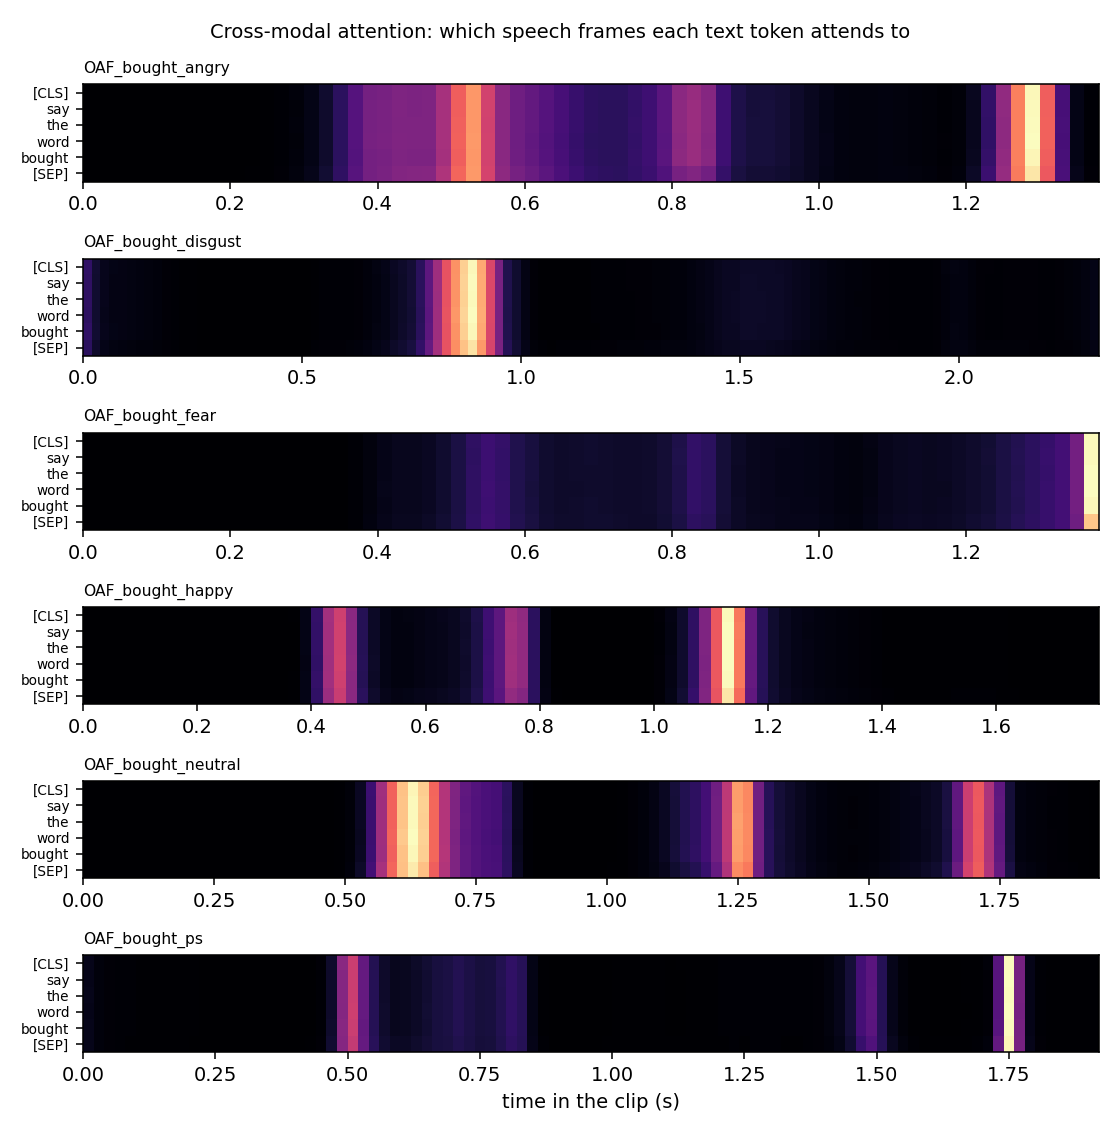
\includegraphics[width=0.66\linewidth]{attention_maps.png}
\caption{Cross-modal attention of six test clips of the word ``bought'' (OAF, seed 0): rows are text tokens,
columns 20\,ms speech frames. All tokens attend to the same few frames.}
\label{fig:attn}
\end{figure}

\section{Limitations}
\begin{itemize}
\item \textbf{Two speakers.} The cross-speaker results rest on one pair of actresses; with two voices a
``new speaker'' test has only two directions, and the seed spread is large ($\pm$ 7--12 points).
\item \textbf{Model selection cannot see the new speaker.} In the cross-speaker splits the validation set comes
from the training speaker and reaches 100\% in every run, so it cannot tell epochs apart, and the chosen epoch is
arbitrary for the other voice. This explains much of the seed spread; a validation set from a third speaker would
fix it, but TESS has only two.
\item \textbf{Acted speech.} TESS emotions are posed and exaggerated, which is why known voices score 99.8\%;
natural speech is far harder.
\item \textbf{Frozen encoders.} Fine-tuning WavLM might improve cross-speaker accuracy but would also overfit 2,000
clips; I kept the encoders frozen to keep the comparison between pipelines fair.
\end{itemize}

\section{Reproducibility}
The code, results and this report are in the repository: \code{models/\{speech,text,fusion\}\_pipeline/}
\code{train.py} and \code{test.py}, shared code in \code{common/}, and \code{scripts/} for features, all runs,
tables and plots, the text bound and the few-shot test. \code{kaggle/TESS\_emotion.ipynb} reproduces everything on
a Kaggle GPU; \code{kaggle/TESS\_emotion\_executed.ipynb} is the run behind these numbers (code build
\code{2391b93e}). \code{kaggle/TESS\_augmentation.ipynb} (build \code{d3fb5e5a}) runs the speaker-augmentation
experiment of Section~\ref{sec:aug}, with features from \code{scripts/extract\_augmented.py}; its results are in
\code{Results\_aug/}.
\code{Results/} holds every run's metrics, predictions, test representations and training log, and the model
weights of seed 0. The README lists the commands.

\end{document}
